\documentclass[12pt]{article}


\usepackage[pdftex,pdfpagelabels,bookmarks,hyperindex,hyperfigures]{hyperref}

\usepackage{graphicx,subcaption,multicol}
\usepackage[margin=1in]{geometry}
\usepackage{float}
\usepackage{adjustbox}
\usepackage[table]{xcolor}
\usepackage{cite}
\usepackage{amsmath,amssymb,amsfonts}
\usepackage{algorithmic}
\usepackage{graphicx}
\usepackage{textcomp}
\usepackage{xcolor}
\usepackage{pgfplots}
\usepackage{fancyhdr}
\usepackage{color}
\usepackage{listings}


\setlength{\parskip}{1em} % Add spacing between paragraphs
\setlength{\parindent}{0em} % Remove indentation at the start of paragraphs


\pagestyle{fancy}
\fancyhf{} % Clear all headers/footers
\lhead{Project Step 3}
\rfoot{\thepage}
\renewcommand{\headrulewidth}{0.4pt}
\renewcommand{\footrulewidth}{0pt}


% --- Title and TOC ---

\begin{document}

\title{4P78 Project Step 3}
\author{
    Parker TenBroeck 7376726\\
    pt21zs@brocku.ca
}
\date{\today}

\makeatletter
\begin{titlepage}
	\def \LOGOPATH {brock.jpg}
	\def \UNIVERSITY {Brock University}
	\def \FACULTY {Faculty of Mathematics \& Science}
	\def \DEPARTMENT {Department of Computer Science}
	\def \COURSETITLE {COSC 3P93: Parallel Computing}
	\def \SUPERVISOR {Robson De Grande}
	
	
	\vfill
	\begin{center}
		\includegraphics[width=0.6\textwidth]{brock.jpg}
		\fontsize{14pt}{14pt}\selectfont
		\vfill
		\UNIVERSITY \\
		\FACULTY \\
		\DEPARTMENT \\
		\vfill
		\fontsize{18pt}{18pt}\selectfont
		\textbf{\COURSETITLE} \\[0.5cm]
		\textbf{\@title}
		\vfill
		\fontsize{14pt}{14pt}\selectfont
		Prepared By: \\[0.5cm]
		
		\begin{tabular}[t]{c}
			\@author
		\end{tabular}\par
	
	    \vfill
		Instructor: \\
		\SUPERVISOR
		\vfill
		\@date
	\end{center}
\end{titlepage}
\makeatother

\newpage

\section{Intro}
My topic is rendering of triangle meshes. \\

This topic is explored in great depth and has a wide array of different techniques and optimizations to produce varying levels of realism. Additionally parallelization often goes hand in hand when talking about these techniques as they are designed for GPUs. \\

I heavily relied on material and techniques talked about on the Learn OpenGL\cite{learn-open-gl} website.\\

The final rendered results for all three scenes (1080) can be seen here \href{https://cosc.brocku.ca/~pt21zs/demo.html}{demo}

\section{Algorithm Overview}

There are a 4 major steps involved in this process

\begin{enumerate}
	\item Transforming from local space to clip space through the Projection, View, and Model matrices
	\item Clipping out of view verticies and triangles.
	\item Rasterizing triangles to the frame buffer
	\item Performing per fragment(pixel) lighting 
\end{enumerate}


\subsection{Projection}
the projection matrix translates coordinates into clip space \eqref{clip-bounds}.
\begin{gather*}\begin{align}
		&fov = \text{the field of view for our camera} \notag\\
		&far = \text{the farthest point our camera can see} \notag\\
		&near = \text{the closest point our camera can see} \notag\\
		&M_{projection} = 
		\begin{bmatrix} 
			\frac{1}{aspect*\tan(\frac{fov}2)}&0&0&0\\
			0&\frac{1}{\tan(\frac{fov}2)}&0&0\\
			0&0&-\frac{far+near}{far-near}&-\frac{2\times far \times near}{far-near}\\
			0&0&-1&0
		\end{bmatrix}
\end{align}\end{gather*}


\subsection{View}
The view matrix transforms world space coordinates into view space coordinates where x is left and right, y is up and down, and z is depth.
\begin{gather*}\begin{align}
		&P_{target} = \text{Where the camera is looking} \notag\\
		&P_{eye} = \text{Where the camera is} \notag\\
		&\overrightarrow{V_{world\hspace{0.2em}up}} = \text{the up direction of the world }\left\langle \begin{matrix}0&1&0\end{matrix} \right\rangle \notag\\
		&\overrightarrow{V_{cam\hspace{0.2em}forward}} = \left\langle P_{target}-P_{eye} \right\rangle \notag\\
		&\overrightarrow{V_{cam\hspace{0.2em}right}} = \left\langle \overrightarrow{V_{cam\hspace{0.2em}forward}}\times  \overrightarrow{V_{world\hspace{0.2em}up}}\right\rangle \notag\\
		&\overrightarrow{V_{cam\hspace{0.2em}up}} = \left\langle \overrightarrow{V_{cam\hspace{0.2em}right}}\times  \overrightarrow{V_{cam\hspace{0.2em}forward}}\right\rangle \notag\\
		&M_{view}= 
		\begin{bmatrix}
			\overrightarrow{V_{cam\hspace{0.2em}right}}_x&\overrightarrow{V_{cam\hspace{0.2em}right}}_y&\overrightarrow{V_{cam\hspace{0.2em}right}}_z&\overrightarrow{V_{cam\hspace{0.2em}right}}\cdot P_{eye}\\
			\overrightarrow{V_{cam\hspace{0.2em}up}}_x&\overrightarrow{V_{cam\hspace{0.2em}up}}_y&\overrightarrow{V_{cam\hspace{0.2em}up}}_z&\overrightarrow{V_{cam\hspace{0.2em}up}}\cdot P_{eye}\\
			-\overrightarrow{V_{cam\hspace{0.2em}forward}}_x&-\overrightarrow{V_{cam\hspace{0.2em}forward}}_y&-\overrightarrow{V_{cam\hspace{0.2em}forward}}_z&\overrightarrow{V_{cam\hspace{0.2em}forward}}\cdot P_{eye}\\
			0&0&0&1
		\end{bmatrix}
\end{align}\end{gather*}

\subsection{Model}

The model matrix transforms coordinates from their local model positions to world space. 
\begin{gather}\begin{align}
		&P_{pos} = \text{world space location of the object} \notag\\
		&\overrightarrow{V_{scale}} = \text{x, y, z scale of object} \notag\\
		&A_{rotation} = \text{euler angles of objects rotation, raw,pitch,roll} \notag\\
		%
		&M_{yaw} = \begin{bmatrix}
			\cos(yaw)&-\sin(yaw)&0\\
			\sin(yaw)&\cos(yaw)&0\\
			0&0&1
		\end{bmatrix} \notag\\
		&M_{pitch} = \begin{bmatrix}
			\cos{pitch}&0&\sin(pitch)\\
			0&1&0\\
			-\sin{pitch}&0&\cos{pitch}
		\end{bmatrix} \notag\\
		&M_{roll} = \begin{bmatrix}
			1&0&0\\
			0&\cos(roll)&-\sin(roll)\\
			0&\sin(roll)&\cos(roll)
		\end{bmatrix} \notag\\
		%
		&M_{rot} = M_{yaw} \cdot M_{pitch} \cdot M_{roll} \notag \\
		%
		&M_{scale} = \begin{bmatrix}
			\overrightarrow{V_{scale}}_x&0&0\\
			0&\overrightarrow{V_{scale}}_y&0\\
			0&0&\overrightarrow{V_{scale}}_z
		\end{bmatrix} \notag\\
		&M_{rot\hspace{0.2em}scale} = M_{rot}\cdot M_{scale} \notag\\
		&M_{model} = \begin{bmatrix}
			{M_{rot\hspace{0.2em}scale}}_{11}&{M_{rot\hspace{0.2em}scale}}_{12}&{M_{rot\hspace{0.2em}scale}}_{13}&{P_{pos}}_x\\
			{M_{rot\hspace{0.2em}scale}}_{21}&{M_{rot\hspace{0.2em}scale}}_{22}&{M_{rot\hspace{0.2em}scale}}_{23}&{P_{pos}}_y\\
			{M_{rot\hspace{0.2em}scale}}_{31}&{M_{rot\hspace{0.2em}scale}}_{32}&{M_{rot\hspace{0.2em}scale}}_{33}&{P_{pos}}_z\\
			0&0&0&1
		\end{bmatrix}
\end{align}\end{gather}

\subsection{Clip}


\begin{gather*}\begin{aligned}
		V_{world} &= M_{model} \cdot V_{local} \notag\\
		V_{clip} &= M_{projection} \cdot M_{view} \cdot M_{model} \cdot V_{local} \notag\\
		%
		M_{normal} &= {{M_{model}}^{-1}}^T \notag\\
		\left\langle N_{world} \right\rangle &= M_{normal} \cdot \left\langle N_{local} \right\rangle \notag
\end{aligned}\end{gather*}

If the resulting vertex is outside this range it is not visible and can be clipped.
\begin{gather}
	-{V_{clip}}_w \leq {V_{clip}}_x \leq {V_{clip}}_w \label{clip-bounds}\\
	-{V_{clip}}_w \leq {V_{clip}}_y \leq {V_{clip}}_w \notag\\
	-{V_{clip}}_w \leq {V_{clip}}_z \leq {V_{clip}}_w \notag
\end{gather}

\subsection{Depth Perspective}
After clipping each vertexs $x,y,z$ components are divided by their $w$ component to give depth perspective. 

\subsection{Screen Space}
After depth perspective the $x,y$ components are shifted over by $\frac12$ then scaled to the screen width and height.


\subsection{Rasterization}
The rasterizer first finds a bounding box around the screen space coordinates. Then iterates over each pixel in the box finding the barycentric coordinates at that pixel. It uses these to determine if the point is actually in the triangle or not. and if it is find the liniarly interpreted world position, uv, normal, tangent, and bitangent at that point from the three points defining the triangle.

\subsubsection{Perspective Correction}
World position, uv, normal, tangent, and bitangent all need to be perspective corrected when being linearly interpolated during rasterization. This is done by scaling each vector type by $\frac1w$, doing the linear interpolation between face points. then scaling the resulting interpolated vector again by a linearly interpolated $\frac1w$.

\subsection{Fragment}
The fragment uses Binn-Phong shading 
\begin{gather*}\begin{aligned}
		\left\langle \overrightarrow{V_{light\hspace{0.2em}dir}} \right\rangle
		&=
		\left\langle P_{light}-P_{fragment}\right\rangle \notag\\
		%
		\text{light power} 
		&= 
		\frac{\text{light intensity}}{| P_{light}-P_{fragment}|^2}\\
		%
		\text{lambertian} 
		&= \max(0, \left\langle 
		\overrightarrow{V_{light\hspace{0.2em}dir}} \right\rangle \cdot   \left\langle N_{fragment}\right\rangle) \\
		%
		\left\langle\overrightarrow{V_{view\hspace{0.2em}dir}} \right\rangle 
		&= 
		\left\langle P_{eye}-P_{fragment}\right\rangle\\
		%
		\left\langle\overrightarrow{V_{half\hspace{0.2em}dir}} \right\rangle 
		&= 
		\left\langle 
		\left\langle\overrightarrow{V_{view\hspace{0.2em}dir}} \right\rangle
		+
		\left\langle \overrightarrow{V_{light\hspace{0.2em}dir}}  \right\rangle
		\right\rangle \\
		%
		\text{specular} &= \max(0, 
		\left\langle\overrightarrow{V_{half\hspace{0.2em}dir}} \right\rangle
		\cdot
		\left\langle N_{fragment}\right\rangle			
		)^{\text{fragment shininess}}\\
		%
		C_{\text{spec}} &= C_{light}\times \text{specular} \times \text{light power}\\
		%
		C_{\text{diff}} &= C_{light}\times \text{lambertian} \times \text{light power}
\end{aligned}\end{gather*}

\section{Parallel Design}

\definecolor{codebg}{RGB}{245,245,245}
\definecolor{keywordcolor}{RGB}{0,0,180}
\definecolor{commentcolor}{RGB}{0,120,0}
\definecolor{stringcolor}{RGB}{160,0,0}
\definecolor{linenumbercolor}{RGB}{120,120,120}

\lstdefinestyle{cpp}{
	language=C++,
	backgroundcolor=\color{codebg},
	basicstyle=\ttfamily\scriptsize,
	keywordstyle=\color{keywordcolor}\bfseries,
	commentstyle=\color{commentcolor}\itshape,
	stringstyle=\color{stringcolor},
	numbers=left,
	numberstyle=\scriptsize\color{linenumbercolor},
	stepnumber=1,
	numbersep=8pt,
	tabsize=2,
	showstringspaces=false,
	breaklines=true,
	frame=single,
	rulecolor=\color{black},
	captionpos=b,
	keepspaces=true,
	columns=flexible
}

\subsection{OpenMP}


Each fragment(pixel) has no dependencies and each fragment performs the same computation so we can statically split the frame up and run it in parallel.

\begin{lstlisting}[language=C++, style=cpp]
	void fragment(FrameBuffer& frame, const Scene& scene, const ResourceStore& resources) {
		#pragma omp parallel for schedule(static)
		for (usize i = 0; i < frame.size(); i ++) {
			frame[i] = frame[i].fragment_shader(scene, resources);
		}
	}
\end{lstlisting}

The projection for each face also has no dependencies on eachother, the only step is rasterization which can potentially have multiple threads writing to the same pixel at the same time.

\begin{lstlisting}[language=C++, style=cpp]
void render_mesh(FrameBuffer& frame, const Mesh& mesh) {
	#pragma omp parallel for schedule(static)
	for (usize i = 0; i < mesh.faces.size(); ++i) {
		Face face = mesh.faces[i];
		project_rasterize_face(frame, face);
	}
}
\end{lstlisting}

Special consideration, setting pixels from many different threads in the same frame buffer can lead to race conditions and improper pixel writes.\\

The naive solution would be to put a critical zone in the region where we check if the current pixels depth is farther than the new pixels depth. The issue with this is in the vast majority of the time we don't need this critical section. This operation happens millions of times per second so finding a better solution will be hugely beneficial. \\

What if we have a per pixel lock? this solution is better but using a traditional pthread mutex would waste a significant about of time potentially putting an OS thread to sleep if it doesn't immediately aquire it and wastes a ton of space per pixel to store the mutex itself.\\

 Per pixel spin lock? This is better as we know we will only be locking for a single comparason and few bytes written to memory so will only spin for a minimal number of cycles. but we still need extra space for the lock value.\\
 
 Using values already in our pixel. If we use the depth value in our pixel (which can only go from \texttt{0x0} to \texttt{0xFFFFFFFE}) we can use a special value \texttt{0xFFFFFFFF} that signals "this pixel is locked". This is the final idea which lead to the code below\\

\begin{lstlisting}[language=C++, style=cpp]
void set_smaller_depth(Pixel pixel) {
	constexpr u32 LOCK_VALUE = 0xFFFFFFFF;

	const std::atomic<u32>* atomic = &this->depth;
	u32 depth;
	while ((depth = atomic->exchange(LOCK_VALUE, std::memory_order_acquire)) == LOCK_VALUE){}
	if (depth > pixel.depth) {
		depth = pixel.depth;
		std::memcpy(this, &pixel, sizeof(Pixel)-sizeof(pixel.depth));
	}
	atomic->store(depth, std::memory_order_release);
}
\end{lstlisting}

This works! it has very little to no noticable performance impact (less than 1\% difference between runs using OpenMP with a single thread and the serial version). Does not require extra data stored per pixel. and does not serialize writes to different pixels.


\pagebreak
\subsection{OpenMPI}

Coordinator
\begin{lstlisting}[language=C++, style=cpp]
void mpi_coordinator(const Arguments& args) {
	mpi::coordinator_broadcast(args, mpi::Tag::Arguments);
	
	u32 frame = 0;
	u32 outstanding = mpi::worker_count();
	
	while (frame < args.frames || outstanding!=0) {
		auto receiver = mpi::Receiver::probe();
		
		 switch (receiver.type()) {
			case mpi::Tag::FrameComplete: {
				const auto finished_frame = receiver.receive<u32>();
				if (finished_frame == 0xFFFFFFFF) {
					outstanding--;
				}
			}break;
			case mpi::Tag::WorkerReady: 
				if (frame < args.frames) {
					receiver.receive<mpi::Empty>(nullptr).sender(mpi::Tag::BeginFrame).send(frame);
					frame++;
				}else {
					receiver.receive<mpi::Empty>(nullptr).sender(mpi::Tag::BeginFrame).send(0xFFFFFFFF);
				}break;
			case mpi::Tag::LoadFile: {
				auto path = receiver.receive<std::string>();
				auto data = file_load_string(path);
				receiver.sender().send(data);
			}break;
			
			default:break;
		}
	}
}
\end{lstlisting}

Worker
\begin{lstlisting}[language=C++, style=cpp]
void mpi_worker() {
	const auto args = mpi::Receiver::begin(mpi::COORDINATOR, mpi::Tag::Arguments).receive<Arguments>();
	auto game = Game::make_game(args);
	
	while (true) {
		auto receiver = mpi::Sender::begin(mpi::COORDINATOR, mpi::Tag::WorkerReady).send(mpi::Empty{}).receiver(mpi::Tag::BeginFrame);
		u32 frame = receiver.receive<u32>();
		if (frame == 0xFFFFFFFF) {
			receiver.sender(mpi::Tag::FrameComplete).send(frame);
			return;
		}
		game->render();
	}
}
\end{lstlisting}

A custom typesafe wrapper around MPI calls was designed to help make development easier. Send and Receive wrap \texttt{MPI\_Recv} and \texttt{MPI\_Send} and provide the corresponding MPI type, count, and tag.\\

The architecture is a single coordinator and many worker model where the coordinator coordinates which worker renders which frame and is also responsible for serving requested files.\\
The worker is responsible for rendering requested frames and also requesting any resources (textures, model data) if needed from the coordinator.


\section{Performance Testing}

\begin{table}[H]
	\caption{Performance Bench Parameters}
	\centering
	\begin{tabular}{|c|c|}
		\hline
		Resolution& 360x240, 720x480, 1080x1920\\\hline
		Scenes/Triangles& Wavy(7212), Halo(42600), Bricks(752456)\\\hline
		Parallelism& Single Thread, MP/MPI(\#1, \#2, \#4, \#8, \#16)\\\hline
		Frames&300\\\hline
		CPU&AMD Ryzen 9 7950X (32) @ 5.883GHz\\\hline
		OS&NixOS 25.05 (Warbler) x86\_64\\\hline
		RAM&64GiB DDR5 \\\hline
		Compiler&clang version 19\\\hline
	\end{tabular}
	\label{table:performance-720-brick}
\end{table}

\subsection{Reproducibility} 
each scene had 300 different frames rendered to ensure random variations in time were minimal.

\section{Results}

\subsection{Rendering Only}

\begin{figure}[H]
	\centering
	\begin{subfigure}{.475\linewidth}
		\centering
		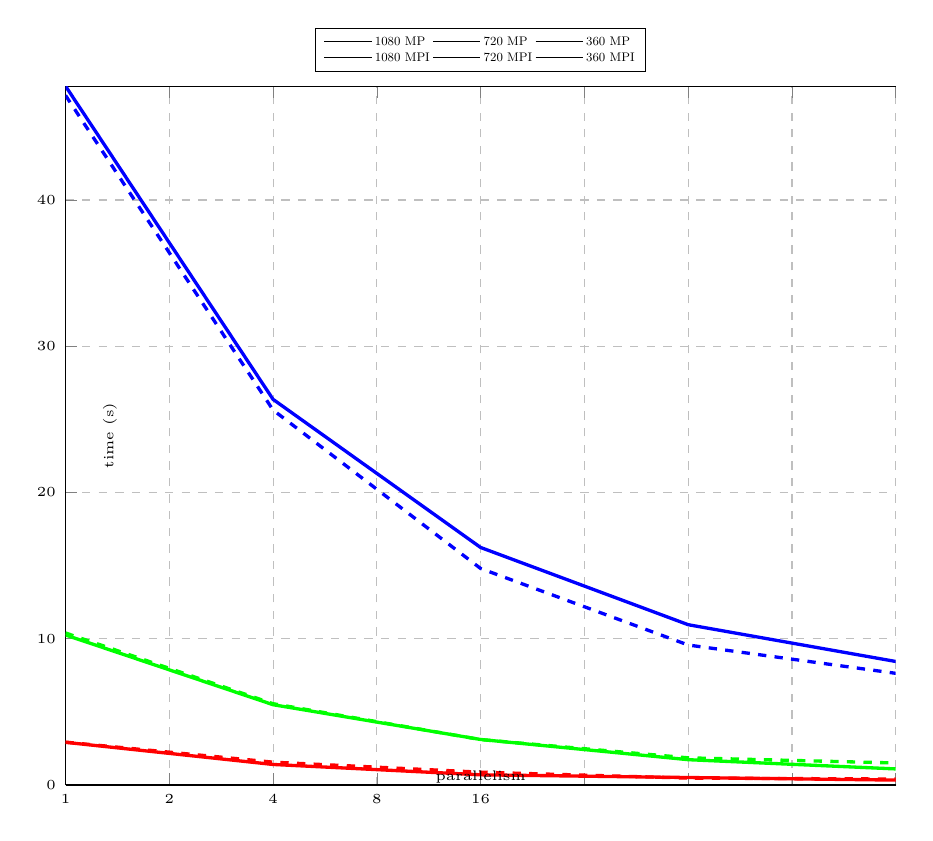
\begin{tikzpicture}[font=\tiny]
\pgfplotsset{
    xmin=0, xmax=4,xticklabels={$0$,$1$,$2$,$4$,$8$,$16$},
 ytick distance=10, 
}

\begin{axis}[
    axis y line*=left,
    ymin=0.0, ymax=47.7888,
xlabel=parallelism,
width=\textwidth,
xlabel style={at={(ticklabel* cs:0.5,3)},anchor=south},
ylabel=time (s),
ylabel style={at={(ticklabel* cs:0.5,-10)},anchor=north},
xmajorgrids=true,
ymajorgrids=true,
grid style=dashed,
legend columns=3,
legend style={nodes={scale=0.5}, at={(0.5,1.02)}, anchor=south},
legend cell align={left}
]

\addlegendimage{/pgfplots/refstyle=mp1080}\addlegendentry{\small 1080 MP}
\addlegendimage{/pgfplots/refstyle=mp720}\addlegendentry{\small 720 MP}
\addlegendimage{/pgfplots/refstyle=mp360}\addlegendentry{\small 360 MP}

\addlegendimage{/pgfplots/refstyle=mpi1080}\addlegendentry{\small 1080 MPI}
\addlegendimage{/pgfplots/refstyle=mpi720}\addlegendentry{\small 720 MPI}
\addlegendimage{/pgfplots/refstyle=mpi360}\addlegendentry{\small 360 MPI}

\addplot[very thick,blue]
coordinates{(0,47.7888)(1,26.368)(2,16.2411)(3,10.9613)(4,8.44716)}; \label{mp1080}

\addplot[very thick,green]
coordinates{(0,10.258)(1,5.49153)(2,3.11437)(3,1.73241)(4,1.1007)}; \label{mp720}

\addplot[very thick,red]
coordinates{(0,2.92)(1,1.40577)(2,0.697979)(3,0.512867)(4,0.336725)}; \label{mp360}

\addplot[blue,dashed,very thick]
coordinates{(0,47.1539)(1,25.6388)(2,14.8047)(3,9.57218)(4,7.63727)}; \label{mpi1080}

\addplot[green,dashed,very thick]
coordinates{(0,10.3965)(1,5.55979)(2,3.10742)(3,1.85908)(4,1.50748)};\label{mpi720}

\addplot[red,dashed,very thick]
coordinates{(0,2.9328)(1,1.56314)(2,0.876581)(3,0.473731)(4,0.409177)    };\label{mpi360}
\end{axis}

\end{tikzpicture}

		\caption{Wavy}
		\label{plot:wavy_render}
	\end{subfigure}\hfill
	\begin{subfigure}{.475\linewidth}
		\centering
		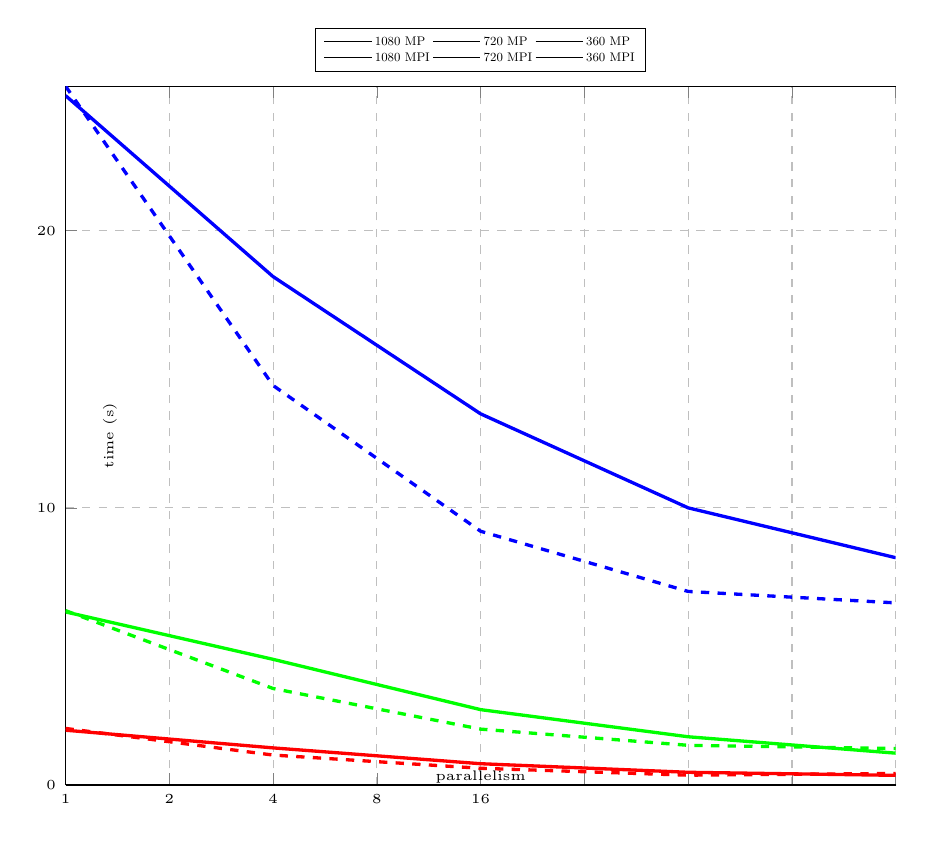
\begin{tikzpicture}[font=\tiny]
\pgfplotsset{
    xmin=0, xmax=4,xticklabels={$0$,$1$,$2$,$4$,$8$,$16$},
 ytick distance=10, 
}

\begin{axis}[
    axis y line*=left,
    ymin=0.0, ymax=25.2181,
xlabel=parallelism,
width=\textwidth,
xlabel style={at={(ticklabel* cs:0.5,3)},anchor=south},
ylabel=time (s),
ylabel style={at={(ticklabel* cs:0.5,-10)},anchor=north},
xmajorgrids=true,
ymajorgrids=true,
grid style=dashed,
legend columns=3,
legend style={nodes={scale=0.5}, at={(0.5,1.02)}, anchor=south},
legend cell align={left}
]

\addlegendimage{/pgfplots/refstyle=mp1080}\addlegendentry{\small 1080 MP}
\addlegendimage{/pgfplots/refstyle=mp720}\addlegendentry{\small 720 MP}
\addlegendimage{/pgfplots/refstyle=mp360}\addlegendentry{\small 360 MP}

\addlegendimage{/pgfplots/refstyle=mpi1080}\addlegendentry{\small 1080 MPI}
\addlegendimage{/pgfplots/refstyle=mpi720}\addlegendentry{\small 720 MPI}
\addlegendimage{/pgfplots/refstyle=mpi360}\addlegendentry{\small 360 MPI}

\addplot[very thick,blue]
coordinates{(0,24.8758)(1,18.3429)(2,13.3923)(3,10.0002)(4,8.20132)}; \label{mp1080}

\addplot[very thick,green]
coordinates{(0,6.2457)(1,4.53517)(2,2.71961)(3,1.74103)(4,1.14969)}; \label{mp720}

\addplot[very thick,red]
coordinates{(0,1.97769)(1,1.33981)(2,0.76862)(3,0.459241)(4,0.349303)}; \label{mp360}

\addplot[blue,dashed,very thick]
coordinates{(0,25.2181)(1,14.4159)(2,9.15593)(3,6.98393)(4,6.57171)}; \label{mpi1080}

\addplot[green,dashed,very thick]
coordinates{(0,6.29262)(1,3.48258)(2,2.01697)(3,1.43255)(4,1.319)};\label{mpi720}

\addplot[red,dashed,very thick]
coordinates{(0,2.04247)(1,1.0813)(2,0.604167)(3,0.355497)(4,0.417648)    };\label{mpi360}
\end{axis}

\end{tikzpicture}

		\caption{Halo}
		\label{plot:halo_render}
	\end{subfigure}
	\medskip
	\begin{subfigure}{.475\linewidth}
		\centering
		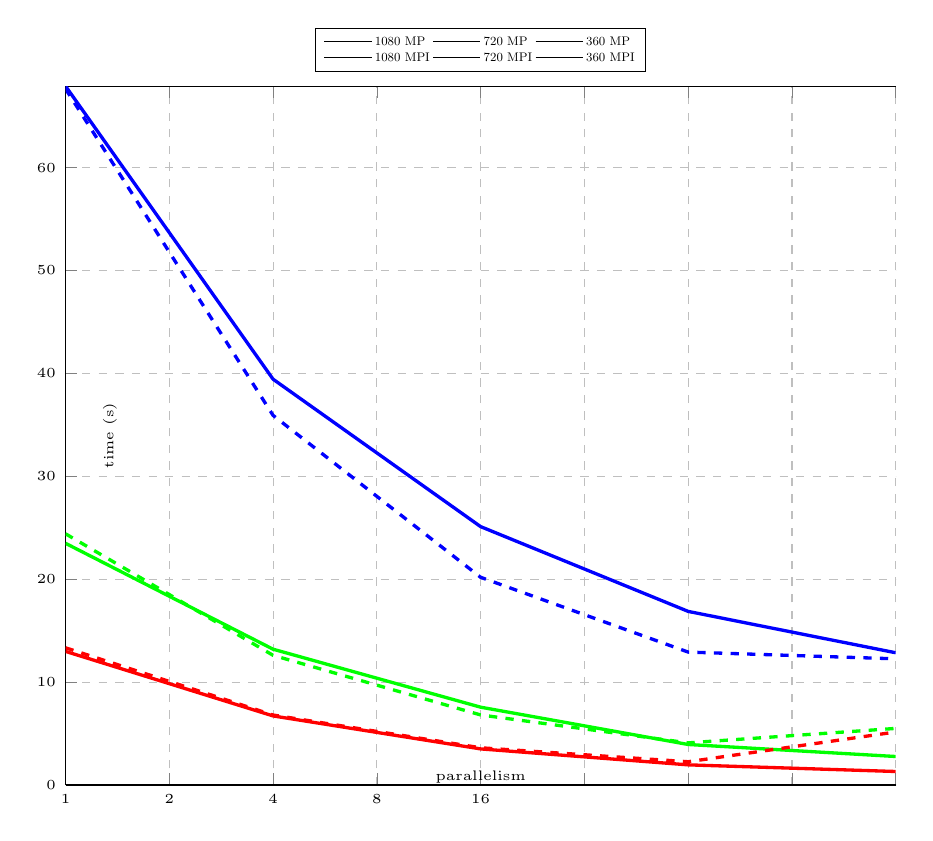
\begin{tikzpicture}[font=\tiny]
\pgfplotsset{
    xmin=0, xmax=4,xticklabels={$0$,$1$,$2$,$4$,$8$,$16$},
 ytick distance=10, 
}

\begin{axis}[
    axis y line*=left,
    ymin=0.0, ymax=67.9241,
xlabel=parallelism,
width=\textwidth,
xlabel style={at={(ticklabel* cs:0.5,3)},anchor=south},
ylabel=time (s),
ylabel style={at={(ticklabel* cs:0.5,-10)},anchor=north},
xmajorgrids=true,
ymajorgrids=true,
grid style=dashed,
legend columns=3,
legend style={nodes={scale=0.5}, at={(0.5,1.02)}, anchor=south},
legend cell align={left}
]

\addlegendimage{/pgfplots/refstyle=mp1080}\addlegendentry{\small 1080 MP}
\addlegendimage{/pgfplots/refstyle=mp720}\addlegendentry{\small 720 MP}
\addlegendimage{/pgfplots/refstyle=mp360}\addlegendentry{\small 360 MP}

\addlegendimage{/pgfplots/refstyle=mpi1080}\addlegendentry{\small 1080 MPI}
\addlegendimage{/pgfplots/refstyle=mpi720}\addlegendentry{\small 720 MPI}
\addlegendimage{/pgfplots/refstyle=mpi360}\addlegendentry{\small 360 MPI}

\addplot[very thick,blue]
coordinates{(0,67.9241)(1,39.439)(2,25.112)(3,16.8739)(4,12.855)}; \label{mp1080}

\addplot[very thick,green]
coordinates{(0,23.4918)(1,13.2002)(2,7.56573)(3,3.93965)(4,2.77215)}; \label{mp720}

\addplot[very thick,red]
coordinates{(0,12.989)(1,6.71582)(2,3.51082)(3,1.96055)(4,1.31552)}; \label{mp360}

\addplot[blue,dashed,very thick]
coordinates{(0,67.6635)(1,35.9213)(2,20.1885)(3,12.9198)(4,12.2649)}; \label{mpi1080}

\addplot[green,dashed,very thick]
coordinates{(0,24.4168)(1,12.6052)(2,6.81128)(3,4.09828)(4,5.50361)};\label{mpi720}

\addplot[red,dashed,very thick]
coordinates{(0,13.3373)(1,6.80444)(2,3.62096)(3,2.26423)(4,5.15598)    };\label{mpi360}
\end{axis}

\end{tikzpicture}

		\caption{Bricks}
		\label{plot:bricks_render}
	\end{subfigure}
	\caption{Scene Render Times}
	\label{plot:render}
\end{figure}


\begin{figure}[H]
	\centering
	\newcommand{\SE}[2]{\footnotesize \(\begin{aligned}S&=#1\times \\[-5pt] E&=#2\% \end{aligned}\)}
\begin{tabular}{l|c c c c}
&2&4&8&16\\
\hline
Bricks 360&\SE{1.93}{96.70}&\SE{3.70}{92.49}&\SE{6.63}{82.81}&\SE{9.87}{61.71}\\
Bricks 720&\SE{1.78}{88.98}&\SE{3.11}{77.63}&\SE{5.96}{74.54}&\SE{8.47}{52.96}\\
Bricks 1080&\SE{1.72}{86.11}&\SE{2.70}{67.62}&\SE{4.03}{50.32}&\SE{5.28}{33.02}\\
Halo 360&\SE{1.48}{73.80}&\SE{2.57}{64.33}&\SE{4.31}{53.83}&\SE{5.66}{35.39}\\
Halo 720&\SE{1.38}{68.86}&\SE{2.30}{57.41}&\SE{3.59}{44.84}&\SE{5.43}{33.95}\\
Halo 1080&\SE{1.36}{67.81}&\SE{1.86}{46.44}&\SE{2.49}{31.09}&\SE{3.03}{18.96}\\
Wavy 360&\SE{2.08}{103.86}&\SE{4.18}{104.59}&\SE{5.69}{71.17}&\SE{8.67}{54.20}\\
Wavy 720&\SE{1.87}{93.40}&\SE{3.29}{82.34}&\SE{5.92}{74.02}&\SE{9.32}{58.25}\\
Wavy 1080&\SE{1.81}{90.62}&\SE{2.94}{73.56}&\SE{4.36}{54.50}&\SE{5.66}{35.36}\\
Average&\SE{1.71}{85.57}&\SE{2.96}{74.05}&\SE{4.77}{59.68}&\SE{6.82}{42.64}\\
\end{tabular}
	\caption{MP Render Time}
	\label{table:mp_render}
\end{figure}


\begin{figure}[H]
	\centering
	\newcommand{\SE}[2]{\footnotesize \(\begin{aligned}S&=#1\times \\[-5pt] E&=#2\% \end{aligned}\)}
\begin{tabular}{l|c c c c}
&2&4&8&16\\
\hline
Bricks 360&\SE{1.96}{98.00}&\SE{3.68}{92.08}&\SE{5.89}{73.63}&\SE{2.59}{16.17}\\
Bricks 720&\SE{1.94}{96.85}&\SE{3.58}{89.62}&\SE{5.96}{74.47}&\SE{4.44}{27.73}\\
Bricks 1080&\SE{1.88}{94.18}&\SE{3.35}{83.79}&\SE{5.24}{65.46}&\SE{5.52}{34.48}\\
Halo 360&\SE{1.89}{94.45}&\SE{3.38}{84.52}&\SE{5.75}{71.82}&\SE{4.89}{30.57}\\
Halo 720&\SE{1.81}{90.34}&\SE{3.12}{78.00}&\SE{4.39}{54.91}&\SE{4.77}{29.82}\\
Halo 1080&\SE{1.75}{87.47}&\SE{2.75}{68.86}&\SE{3.61}{45.14}&\SE{3.84}{23.98}\\
Wavy 360&\SE{1.88}{93.81}&\SE{3.35}{83.64}&\SE{6.19}{77.39}&\SE{7.17}{44.80}\\
Wavy 720&\SE{1.87}{93.50}&\SE{3.35}{83.64}&\SE{5.59}{69.90}&\SE{6.90}{43.10}\\
Wavy 1080&\SE{1.84}{91.96}&\SE{3.19}{79.63}&\SE{4.93}{61.58}&\SE{6.17}{38.59}\\
Average&\SE{1.87}{93.40}&\SE{3.31}{82.64}&\SE{5.28}{66.03}&\SE{5.14}{32.14}\\
\end{tabular}
	\caption{MPI Render Time}
	\label{table:mpi_render}
\end{figure}



\subsection{Rendering And Resource Loading}

\begin{figure}[H]
	\centering
	\begin{subfigure}{.475\linewidth}
		\centering
		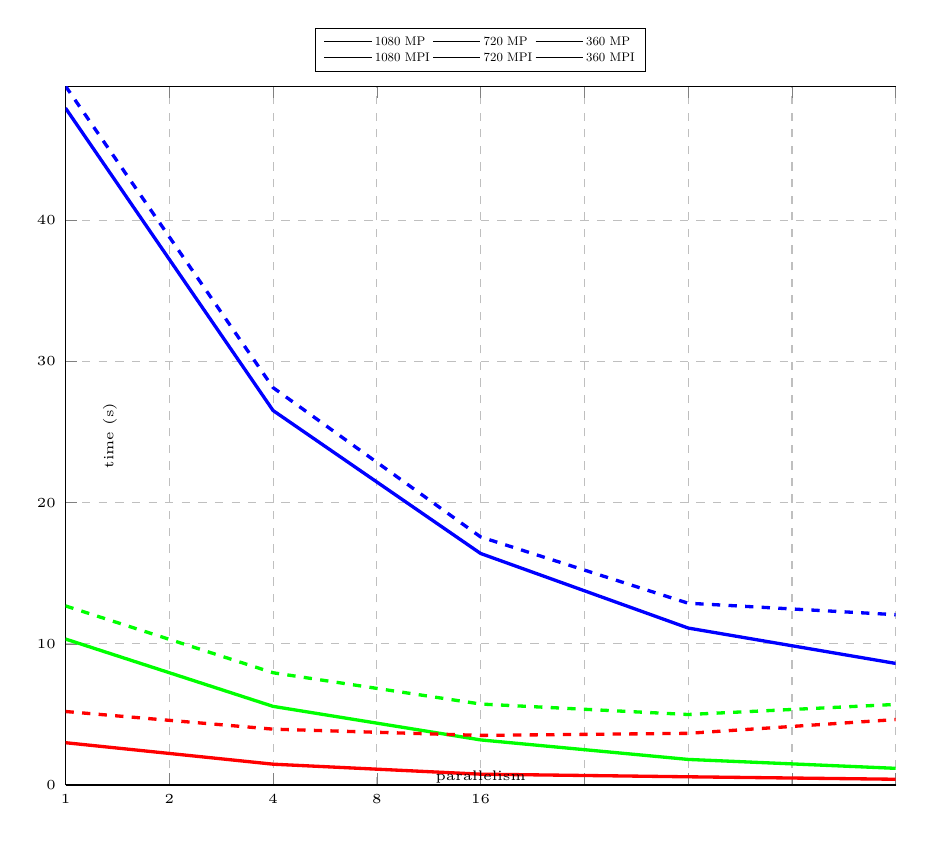
\begin{tikzpicture}[font=\tiny]
\pgfplotsset{
    xmin=0, xmax=4,xticklabels={$0$,$1$,$2$,$4$,$8$,$16$},
 ytick distance=10, 
}

\begin{axis}[
    axis y line*=left,
    ymin=0.0, ymax=49.500108572,
xlabel=parallelism,
width=\textwidth,
xlabel style={at={(ticklabel* cs:0.5,3)},anchor=south},
ylabel=time (s),
ylabel style={at={(ticklabel* cs:0.5,-10)},anchor=north},
xmajorgrids=true,
ymajorgrids=true,
grid style=dashed,
legend columns=3,
legend style={nodes={scale=0.5}, at={(0.5,1.02)}, anchor=south},
legend cell align={left}
]

\addlegendimage{/pgfplots/refstyle=mp1080}\addlegendentry{\small 1080 MP}
\addlegendimage{/pgfplots/refstyle=mp720}\addlegendentry{\small 720 MP}
\addlegendimage{/pgfplots/refstyle=mp360}\addlegendentry{\small 360 MP}

\addlegendimage{/pgfplots/refstyle=mpi1080}\addlegendentry{\small 1080 MPI}
\addlegendimage{/pgfplots/refstyle=mpi720}\addlegendentry{\small 720 MPI}
\addlegendimage{/pgfplots/refstyle=mpi360}\addlegendentry{\small 360 MPI}

\addplot[very thick,blue]
coordinates{(0,47.942430347)(1,26.52299607)(2,16.397328664)(3,11.117000798)(4,8.611362281)}; \label{mp1080}

\addplot[very thick,green]
coordinates{(0,10.338515062)(1,5.570604907)(2,3.195023798)(3,1.813024517)(4,1.18229197)}; \label{mp720}

\addplot[very thick,red]
coordinates{(0,2.997587158)(1,1.47629772)(2,0.768837664)(3,0.58338612)(4,0.408949377)}; \label{mp360}

\addplot[blue,dashed,very thick]
coordinates{(0,49.500108572)(1,28.143107966)(2,17.56904276)(3,12.875771632)(4,12.063108207)}; \label{mpi1080}

\addplot[green,dashed,very thick]
coordinates{(0,12.685091108)(1,7.951905266)(2,5.736529412)(3,4.994016299)(4,5.70861979)};\label{mpi720}

\addplot[red,dashed,very thick]
coordinates{(0,5.207041628)(1,3.957372751)(2,3.514461662)(3,3.661203684)(4,4.636759706)    };\label{mpi360}
\end{axis}

\end{tikzpicture}

		\caption{Wavy}
		\label{plot:wavy_all}
	\end{subfigure}\hfill
	\begin{subfigure}{.475\linewidth}
		\centering
		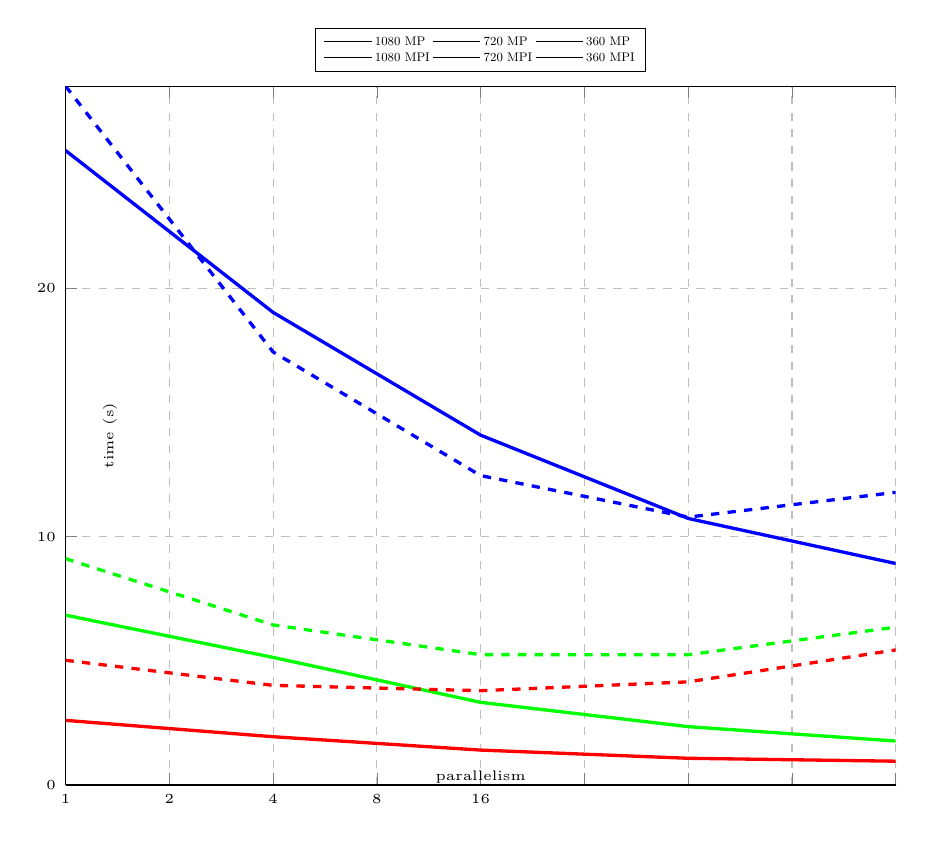
\begin{tikzpicture}[font=\tiny]
\pgfplotsset{
    xmin=0, xmax=4,xticklabels={$0$,$1$,$2$,$4$,$8$,$16$},
 ytick distance=10, 
}

\begin{axis}[
    axis y line*=left,
    ymin=0.0, ymax=28.145487433,
xlabel=parallelism,
width=\textwidth,
xlabel style={at={(ticklabel* cs:0.5,3)},anchor=south},
ylabel=time (s),
ylabel style={at={(ticklabel* cs:0.5,-10)},anchor=north},
xmajorgrids=true,
ymajorgrids=true,
grid style=dashed,
legend columns=3,
legend style={nodes={scale=0.5}, at={(0.5,1.02)}, anchor=south},
legend cell align={left}
]

\addlegendimage{/pgfplots/refstyle=mp1080}\addlegendentry{\small 1080 MP}
\addlegendimage{/pgfplots/refstyle=mp720}\addlegendentry{\small 720 MP}
\addlegendimage{/pgfplots/refstyle=mp360}\addlegendentry{\small 360 MP}

\addlegendimage{/pgfplots/refstyle=mpi1080}\addlegendentry{\small 1080 MPI}
\addlegendimage{/pgfplots/refstyle=mpi720}\addlegendentry{\small 720 MPI}
\addlegendimage{/pgfplots/refstyle=mpi360}\addlegendentry{\small 360 MPI}

\addplot[very thick,blue]
coordinates{(0,25.551531212)(1,19.032699433)(2,14.088536191)(3,10.73390033)(4,8.919271195)}; \label{mp1080}

\addplot[very thick,green]
coordinates{(0,6.839857795)(1,5.139338144)(2,3.328913082)(3,2.350491653)(4,1.771118193)}; \label{mp720}

\addplot[very thick,red]
coordinates{(0,2.603659031)(1,1.94475965)(2,1.40724373)(3,1.076569981)(4,0.958953761)}; \label{mp360}

\addplot[blue,dashed,very thick]
coordinates{(0,28.145487433)(1,17.439509009)(2,12.460023623)(3,10.787702598)(4,11.784487771)}; \label{mpi1080}

\addplot[green,dashed,very thick]
coordinates{(0,9.114140458)(1,6.444869421)(2,5.249999765)(3,5.248349053)(4,6.356409316)};\label{mpi720}

\addplot[red,dashed,very thick]
coordinates{(0,5.022642923)(1,4.01237689)(2,3.798267183)(3,4.153945794)(4,5.439593891)    };\label{mpi360}
\end{axis}

\end{tikzpicture}

		\caption{Halo}
		\label{plot:halo_all}
	\end{subfigure}
	\medskip
	\begin{subfigure}{.475\linewidth}
		\centering
		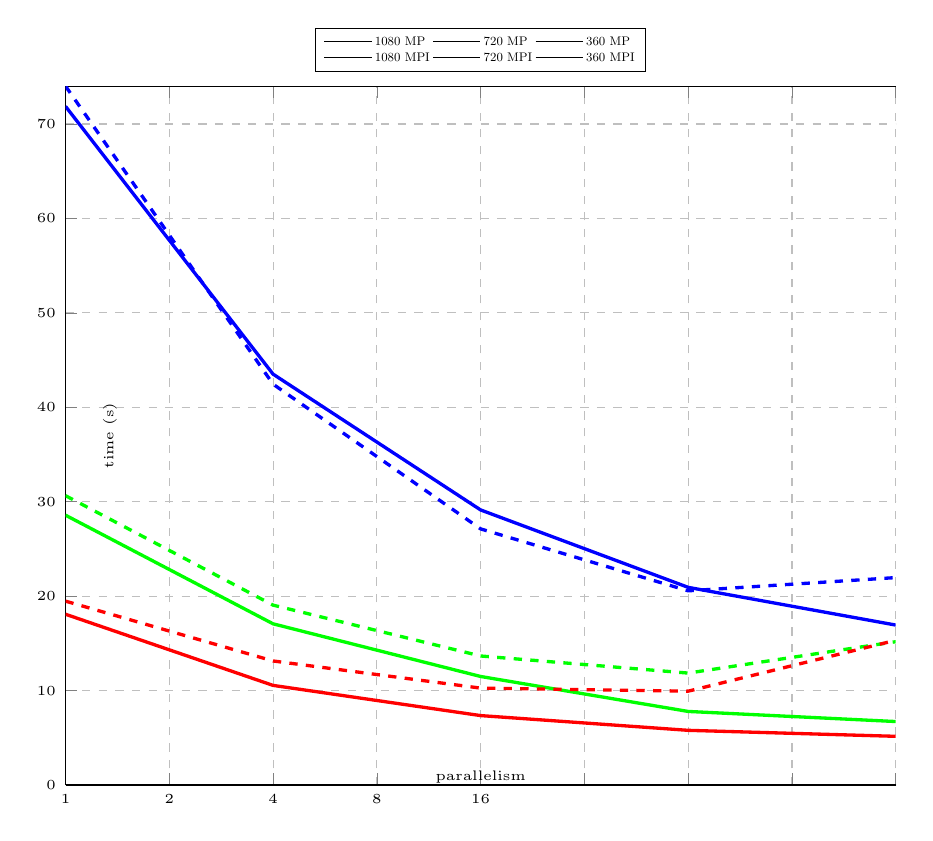
\begin{tikzpicture}[font=\tiny]
\pgfplotsset{
    xmin=0, xmax=4,xticklabels={$0$,$1$,$2$,$4$,$8$,$16$},
 ytick distance=10, 
}

\begin{axis}[
    axis y line*=left,
    ymin=0.0, ymax=74.017875391,
xlabel=parallelism,
width=\textwidth,
xlabel style={at={(ticklabel* cs:0.5,3)},anchor=south},
ylabel=time (s),
ylabel style={at={(ticklabel* cs:0.5,-10)},anchor=north},
xmajorgrids=true,
ymajorgrids=true,
grid style=dashed,
legend columns=3,
legend style={nodes={scale=0.5}, at={(0.5,1.02)}, anchor=south},
legend cell align={left}
]

\addlegendimage{/pgfplots/refstyle=mp1080}\addlegendentry{\small 1080 MP}
\addlegendimage{/pgfplots/refstyle=mp720}\addlegendentry{\small 720 MP}
\addlegendimage{/pgfplots/refstyle=mp360}\addlegendentry{\small 360 MP}

\addlegendimage{/pgfplots/refstyle=mpi1080}\addlegendentry{\small 1080 MPI}
\addlegendimage{/pgfplots/refstyle=mpi720}\addlegendentry{\small 720 MPI}
\addlegendimage{/pgfplots/refstyle=mpi360}\addlegendentry{\small 360 MPI}

\addplot[very thick,blue]
coordinates{(0,71.874419528)(1,43.511030528)(2,29.129720505)(3,20.93201887)(4,16.938586804)}; \label{mp1080}

\addplot[very thick,green]
coordinates{(0,28.574190037)(1,17.070923577)(2,11.493386004)(3,7.790744988)(4,6.721354496)}; \label{mp720}

\addplot[very thick,red]
coordinates{(0,18.084464399)(1,10.549399809)(2,7.3518193)(3,5.790021897)(4,5.155757005)}; \label{mp360}

\addplot[blue,dashed,very thick]
coordinates{(0,74.017875391)(1,42.451153603)(2,27.122364885)(3,20.565048369)(4,21.965591099)}; \label{mpi1080}

\addplot[green,dashed,very thick]
coordinates{(0,30.640323687)(1,19.049641511)(2,13.664910648)(3,11.853540641)(4,15.175364751)};\label{mpi720}

\addplot[red,dashed,very thick]
coordinates{(0,19.472875063)(1,13.136732281)(2,10.260655983)(3,9.938033637)(4,15.324826927)    };\label{mpi360}
\end{axis}

\end{tikzpicture}

		\caption{Bricks}
		\label{plot:bricks_all}
	\end{subfigure}
	\caption{Scene Total Times}
	\label{plot:all}
\end{figure}


\begin{figure}[H]
	\centering
	\newcommand{\SE}[2]{\footnotesize \(\begin{aligned}S&=#1\times \\[-5pt] E&=#2\% \end{aligned}\)}
\begin{tabular}{l|c c c c}
&2&4&8&16\\
\hline
Bricks 360&\SE{1.71}{85.71}&\SE{2.46}{61.50}&\SE{3.12}{39.04}&\SE{3.51}{21.92}\\
Bricks 720&\SE{1.67}{83.69}&\SE{2.49}{62.15}&\SE{3.67}{45.85}&\SE{4.25}{26.57}\\
Bricks 1080&\SE{1.65}{82.59}&\SE{2.47}{61.68}&\SE{3.43}{42.92}&\SE{4.24}{26.52}\\
Halo 360&\SE{1.34}{66.94}&\SE{1.85}{46.25}&\SE{2.42}{30.23}&\SE{2.72}{16.97}\\
Halo 720&\SE{1.33}{66.54}&\SE{2.05}{51.37}&\SE{2.91}{36.37}&\SE{3.86}{24.14}\\
Halo 1080&\SE{1.34}{67.13}&\SE{1.81}{45.34}&\SE{2.38}{29.76}&\SE{2.86}{17.90}\\
Wavy 360&\SE{2.03}{101.52}&\SE{3.90}{97.47}&\SE{5.14}{64.23}&\SE{7.33}{45.81}\\
Wavy 720&\SE{1.86}{92.80}&\SE{3.24}{80.90}&\SE{5.70}{71.28}&\SE{8.74}{54.65}\\
Wavy 1080&\SE{1.81}{90.38}&\SE{2.92}{73.09}&\SE{4.31}{53.91}&\SE{5.57}{34.80}\\
Average&\SE{1.64}{81.92}&\SE{2.58}{64.42}&\SE{3.68}{45.95}&\SE{4.79}{29.92}\\
\end{tabular}
	\caption{MP Total Time}
	\label{table:mp_all}
\end{figure}


\begin{figure}[H]
	\centering
	\newcommand{\SE}[2]{\footnotesize \(\begin{aligned}S&=#1\times \\[-5pt] E&=#2\% \end{aligned}\)}
\begin{tabular}{l|c c c c}
&2&4&8&16\\
\hline
Bricks 360&\SE{1.48}{74.12}&\SE{1.90}{47.45}&\SE{1.96}{24.49}&\SE{1.27}{7.94}\\
Bricks 720&\SE{1.61}{80.42}&\SE{2.24}{56.06}&\SE{2.58}{32.31}&\SE{2.02}{12.62}\\
Bricks 1080&\SE{1.74}{87.18}&\SE{2.73}{68.23}&\SE{3.60}{44.99}&\SE{3.37}{21.06}\\
Halo 360&\SE{1.25}{62.59}&\SE{1.32}{33.06}&\SE{1.21}{15.11}&\SE{0.92}{5.77}\\
Halo 720&\SE{1.41}{70.71}&\SE{1.74}{43.40}&\SE{1.74}{21.71}&\SE{1.43}{8.96}\\
Halo 1080&\SE{1.61}{80.69}&\SE{2.26}{56.47}&\SE{2.61}{32.61}&\SE{2.39}{14.93}\\
Wavy 360&\SE{1.32}{65.79}&\SE{1.48}{37.04}&\SE{1.42}{17.78}&\SE{1.12}{7.02}\\
Wavy 720&\SE{1.60}{79.76}&\SE{2.21}{55.28}&\SE{2.54}{31.75}&\SE{2.22}{13.89}\\
Wavy 1080&\SE{1.76}{87.94}&\SE{2.82}{70.44}&\SE{3.84}{48.06}&\SE{4.10}{25.65}\\
Average&\SE{1.53}{76.58}&\SE{2.08}{51.94}&\SE{2.39}{29.87}&\SE{2.09}{13.09}\\
\end{tabular}
	\caption{MPI Total Time}
	\label{table:mpi_all}
\end{figure}

\section{Analysis}

Time was measured in two ways, "Render Time" which only accounts for the time it takes to render frames. and "Total Time" which accounts for asset loading and resource sharing. Both times were recorded from the exact same runs so the difference is entirely the extra time taken for resource loading.\\

Also importantly, MPI and MP parallelize different parts of the program with differing levels of granularity. 

\subsection{Render Time Only}

The graphs which show these are \ref{plot:all}, \ref{table:mp_all}, and \ref{table:mpi_all}. Interestingly (and unexpectedly) the MPI version performs the same if not better than the MP version in almost all cases. This really caught me off guard when I first looked at the results (so much so I double checked I had the correct data points). But I think a reasonable explanation for this performance difference is true sharing(Cache Coherence). It cannot be false sharing because each pixel is larger than 64 bytes (the cache line on the benchmarking system) and is aligned to 128 byte boundaries. However, in the MP version each thread is rendering over the same image. This means that the L1 cache in particular (for each core) must sync its changes with other cores if they request the same address (to ensure cache coherence). In contrary the MPI implementation has each node(thread in our case) work in its own image. this means that each thread uses its own frame buffer and therefore does not have to constantly sync its L1 cache with other cores when rendering. \\

Even so, once the degree of parallelism reaches 16 the overhead of MPI can be seen as the curves of MPI and MP begin to intersect again.\\

Other than that the graphs and data is about what you'd expect. Both version have almost the exact same performance to begin with. Efficiency drops as parallelism increases. And the effective speed up begins to slow. \\
 
\subsection{Total Time}

These graphs \ref{plot:render}, and tables \ref{table:mp_render} \ref{table:mpi_render} show the total time benchmarks and performance.\\

The MPI versions are almost always slower, with the only exception being in a few of the higher resolution tests.\\

This is due to the overhead of sending/parsing the assets and textures $n$ times where $n$ is the degree of parallelism. Even in the cases where it has runs which are faster at first the performance quickly becomes dominated by the startup time of duplicated work and large data transfers. \\

In both cases the efficiency decreases much quicker compared to render time only which makes sense as the quicker our render time is, the most we are benchmarking "how fast can we read and parse images and model data". 

\subsection{Further Testing}
I did not include this in my report (as I do not have an enviorment to test it in effectively). But MPI and MP can be used together with this program. Since they parallelize different sections of the code it is possible to compile the program with both librries/compiler options enabled(I also tested it to make sure it worked). This could be useful as each MPI node could take full advantage of all local CPU cores on its machine to limit bandwidth/re computation of loading and parsing assets. Additionally each MPI node would only need to request the assets it needs, which if different frames only need  certain assets it could be significant savings in communication overhead.

\section{Building and Runing}

Two seperate build files are provided for each respective compiler \texttt{build\_clang.sh} and \texttt{build\_gcc.sh}. \\
\\
\underline{Important}: to switch between building with gcc or clang you \texttt{must} completely delete all \texttt{cmake-build-*} folders if it has been created previously with the other build script.\\

Also if MP, MPI, or OpenGL is not installed on the build system. that respective build will fail. It will not effect the other builds even if an error is shown when building.\\

Once the project has been built you can perform the same benchmarks in this document by running \texttt{bench.sh}. It will run through all the permutations of the input parameters.\\

Neither the halo nor bricks model is included in the submissions due to licensing reasons though the wavy scene will work just fine. If you wish to run them you must download the models \cite{halo-model} \cite{bricks-model} as OBJ files and place the extracted model in the \texttt{assets} folder nammed \texttt{halo} and \texttt{bricks} respectively.


\nocite{*}
\bibliographystyle{IEEEtran}
\bibliography{references}

\end{document}
